\chapter{Сокрытие в спектральной области}
\section{Дискретное косинусное преобразование}
Дискретное косинусное преобразование (ДКП) --- одно из дискретных преобразований Фурье.
ДКП представляет конечную последовательность в виде суммы функций косинуса,
колеблющихся на разных частотах. ДКП широко используется при обработке сигналов и сжатии данных.
Например, ДКП используется при сжатии в изображениях (JPEG, HEIF), аудиофайлах (Dolby Digital, MP3),
видеофайлах (MPEG, H.26x), в цифровом телевидении (SDTV, HDTV, VOD) и в других.

ДКП является линейным ортогональным преобразованием. Как любое дискретное линейное преобразование,
ДКП можно представить в виде матрицы. Будучи ортоганальным преобразованием, обратное к ДКП преобразование
задает транспонированной матрицей ДКП, домноженной на какой-то коэффициент.

Использование косинусных, а не синусоидальных функций имеет решающее значение для сжатия,
поскольку для аппроксимации типичного сигнала требуется меньше косинусных функций.
ДКП подобно дискретному преобразованию Фурье, но использующее только действительные числа.

Существует 8 стандартных типов ДКП, однако наиболее употребимым является второй тип,
который часто называют просто ДКП (DCT-II).
Формула дискретного косинусного преобразования выглядит так,
как показано в формуле~\ref{eq:simple-dcp}:
\begin{equation} \label{eq:simple-dcp}
    X_k = \sum_{n=0}^{N-1} x_n \cos \left[\frac{\pi}{N} \left(n+\frac{1}{2}\right) k \right] \quad \quad k = 0, \dots, N-1    
\end{equation}
Формула для матрицы преобразования выглядит как формуле~\ref{eq:matrix-dcp}:
\begin{equation} \label{eq:matrix-dcp}
    {DCT}\text{-}2_n= \left[\cos (k(l+\tfrac{1}{2})\tfrac{\pi}{n})\right]_{0\leq k,l<n}    
\end{equation}

Как и в случае быстрого преобразования Фурье, существуют алгоритмы быстрого ДКП преобразования.

DCT-II часто используется для сжатия с потерями благодаря своему свойству уплотнения энерегии:
в типичных случаях большая часть информации, которую содержит сигнал, концентрируется в нескольких
первых коэффициентах разложения.

Существуют так же многомерные ДКП, которые получаются из одномерных путем композиции ДКП по каждому измерению.
Вывод такого преобразования для двумерного случая показан в формуле~\ref{eq:2d-dcp}.
\begin{align}
    X_{k_1,k_2} &= \nonumber
    \sum_{n_1=0}^{N_1-1}
    \left( \sum_{n_2=0}^{N_2-1}
    x_{n_1,n_2} 
    \cos \left[\frac{\pi}{N_2} \left(n_2+\frac{1}{2}\right) k_2 \right]\right)
    \cos \left[\frac{\pi}{N_1} \left(n_1+\frac{1}{2}\right) k_1 \right]\\
    &= \sum_{n_1=0}^{N_1-1}
    \sum_{n_2=0}^{N_2-1}
    x_{n_1,n_2} 
    \cos \left[\frac{\pi}{N_1} \left(n_1+\frac{1}{2}\right) k_1 \right]
    \cos \left[\frac{\pi}{N_2} \left(n_2+\frac{1}{2}\right) k_2 \right] \label{eq:2d-dcp}
\end{align}
Здесь $[x_{n_1,n_2}]$ --- матрица до преобразования, и $[X_{k_1,k_2}]$ --- матрица
после преобразования.
В матричном виде это преобразование может быть представлено так, как показано
в формуле~\ref{eq:2d-matrix-dcp}, где $x$ --- матрица, которую нужно преобразовать.
\begin{equation} \label{eq:2d-matrix-dcp}
    X = ({DCT}\text{-}2_n) x ({DCT}\text{-}2_n ^ T)
\end{equation}
Именно такое преобразование используется при компрессии в JPEG.

\section{JPEG}
JPEG является широко используемым методом сжатия с потерями для цифровых изображений.
Степень сжатия регулируется, что позволяет выбирать между качеством и размером изображения.
JPEG наиболее широко используемый стандарт сжатия изображений в мире и
наиболее используемый формат цифровых изображений.

ДКП лежит в основе сжатия методом JPEG. Как уже говорилось выше,
ДКП был выбран именно благодаря свойству уплотнения энергии. Чтобы прояснить,
о чем идет речь, мной была сделана визуализация преобразования ДКП.

Выберем на изображении область 32x32 пикселя, как показано на рисунке~\ref{img:lenna-eye}.

\begin{figure}[ht!]
    \centering
    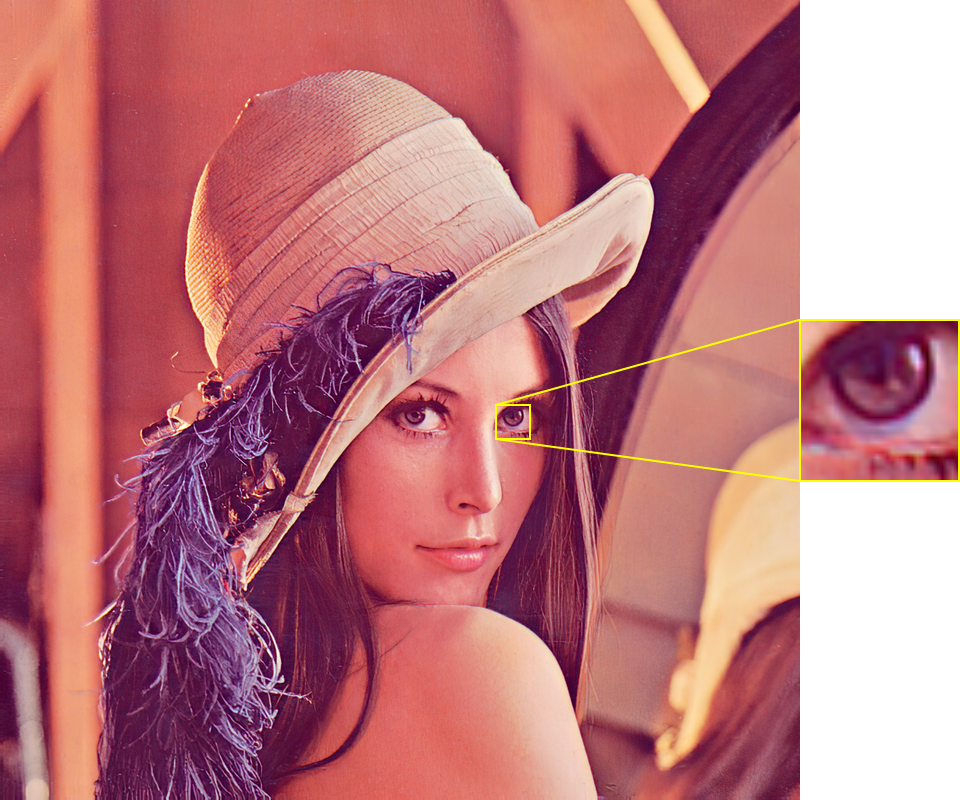
\includegraphics[width=\linewidth]{DCT/Lenna_eye.png}
    \caption{Выбираем область}
    \label{img:lenna-eye}
\end{figure}

%Для простоты будем использовать только синий канал изображения.
Сначала рассмотрим матрицу пикселей как двумерную дискретную функцию.
Расположим координаты так, чтобы в левом верхнем углу
располагался пиксель с координатами $p_{kj}, k = 0, j = 0$.
Визуализацию можно посмотреть на рисунке~\ref{img:pixels-dct}.

\begin{figure}[ht!]
    \centering
    \caption{Визуализация пикселей}
    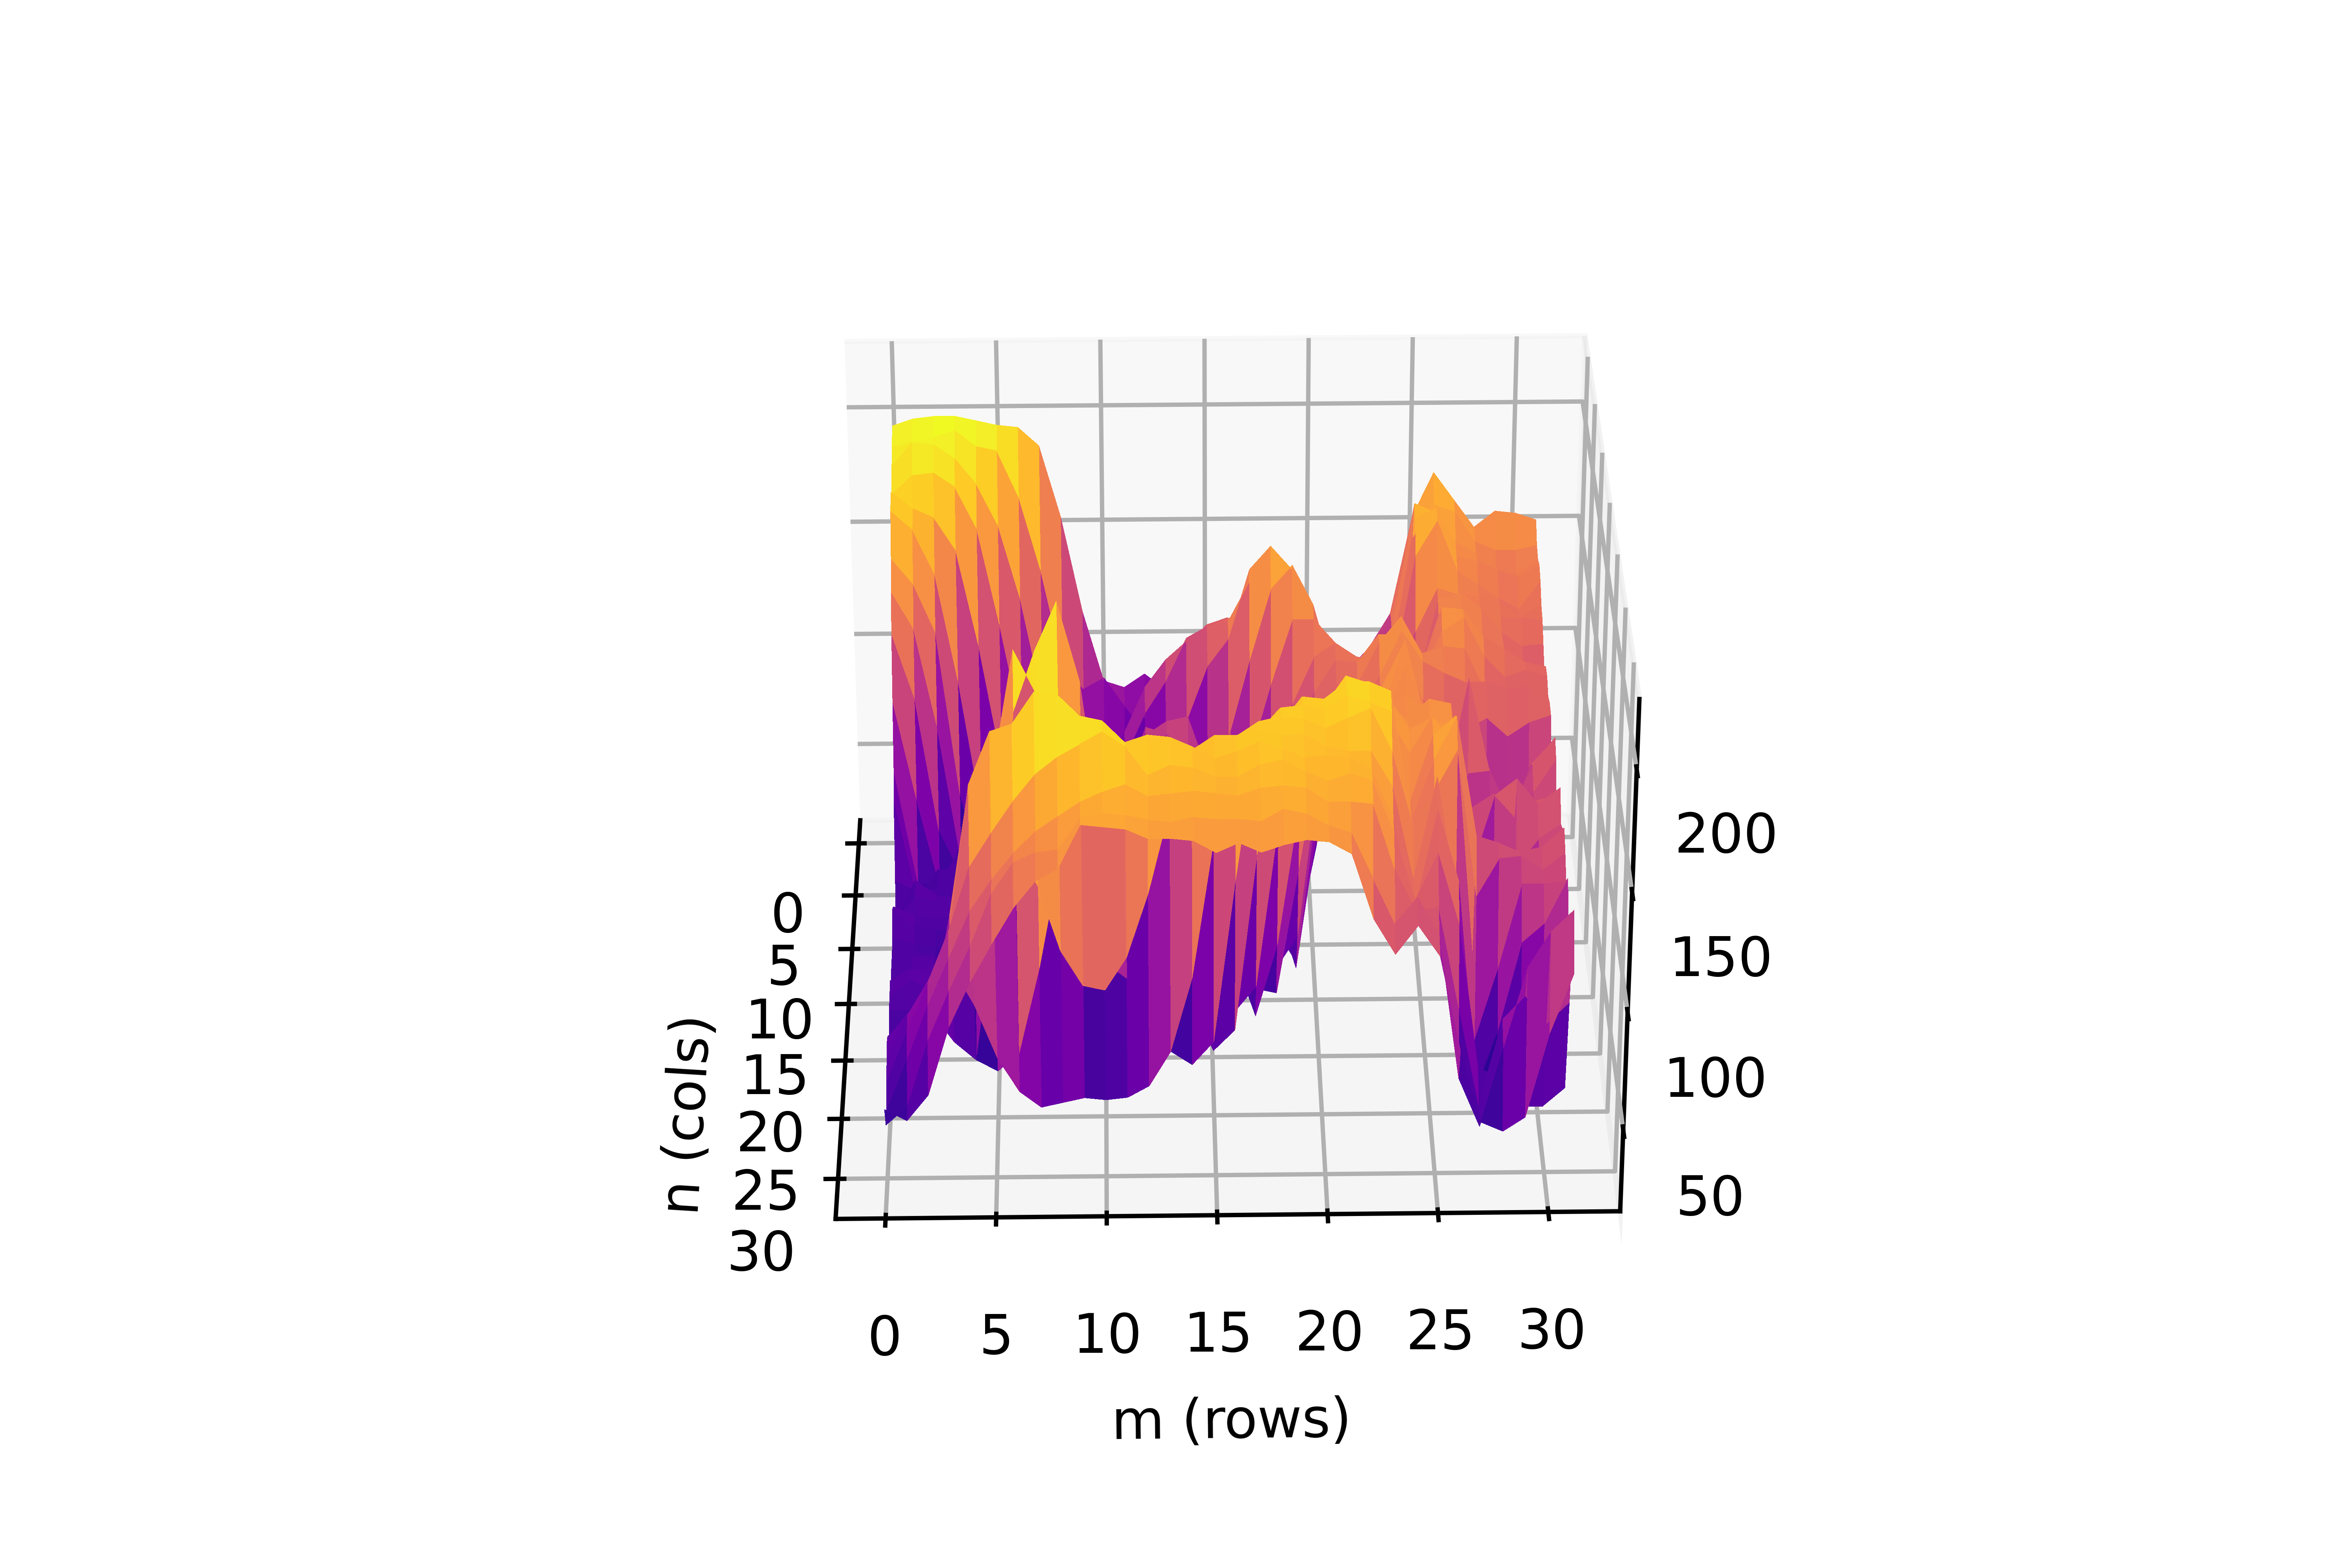
\includegraphics[width=\linewidth]{DCT/pixels.png}
    \label{img:pixels-dct}
\end{figure}

Умножим эту функцию справа на транспонированную матрицу ДКП
по формуле~\ref{eq:2d-matrix-dcp}. Мы получим новую функцию,
которая показана на рисунке~\ref{img:dct-1}.
Таким образом фактически ДКП применилось к каждой строке матрицы.
Из изображения видно, что наибольшие коэффициенты расположены
в нижней части спектра, то есть ближе к нулевому столбцу.

\begin{figure}[ht!]
    \centering
    \caption{После приминения ДКП к строкам матрицы}
    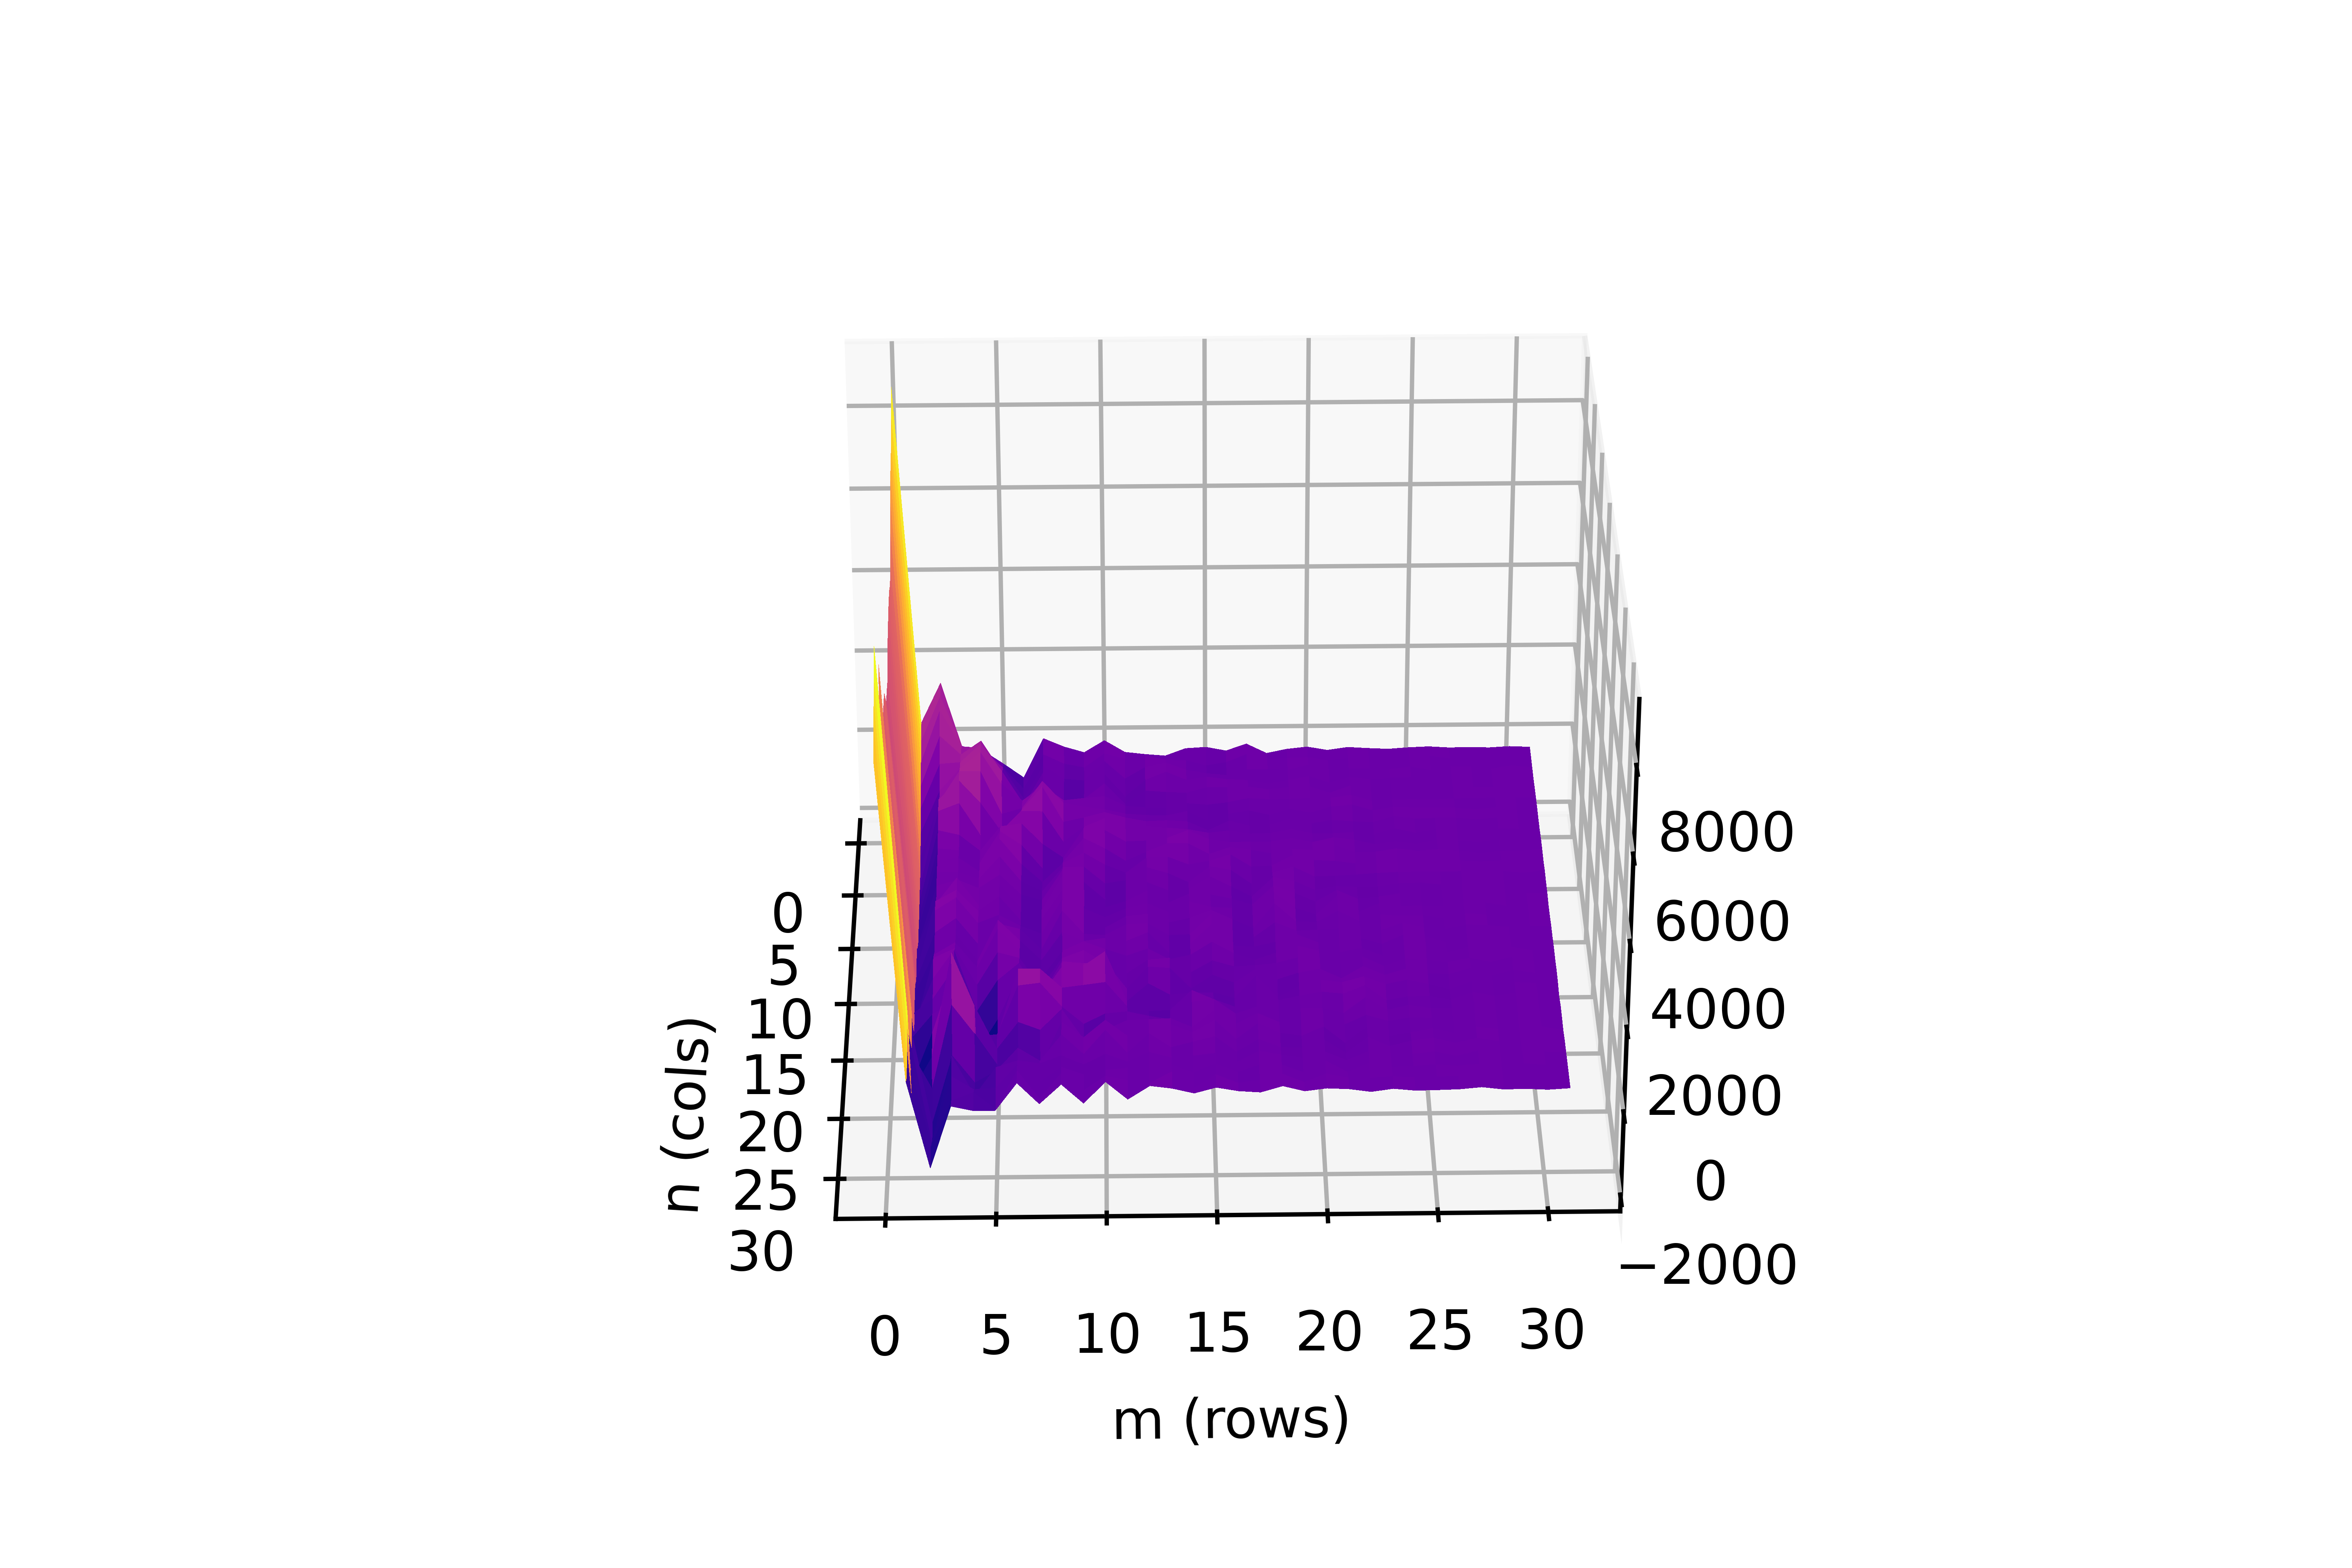
\includegraphics[width=\linewidth]{DCT/dct-1.png}
    \label{img:dct-1}
\end{figure}

К полученной матрице применим ДКП еще раз, в этот раз по столбцам.
В полученной матрице наибольшее значение имеет коэфициент с координатами
$k = 0, j = 0$. Этот коэффициент называется DC-коэффициент.
Остальные коэффициенты называются AC-коэффициентами.
Матрица показана на рисунке~\ref{img:dct-2}.

\begin{figure}[ht!]
    \centering
    \caption{После приминения ДКП к столбцам матрицы}
    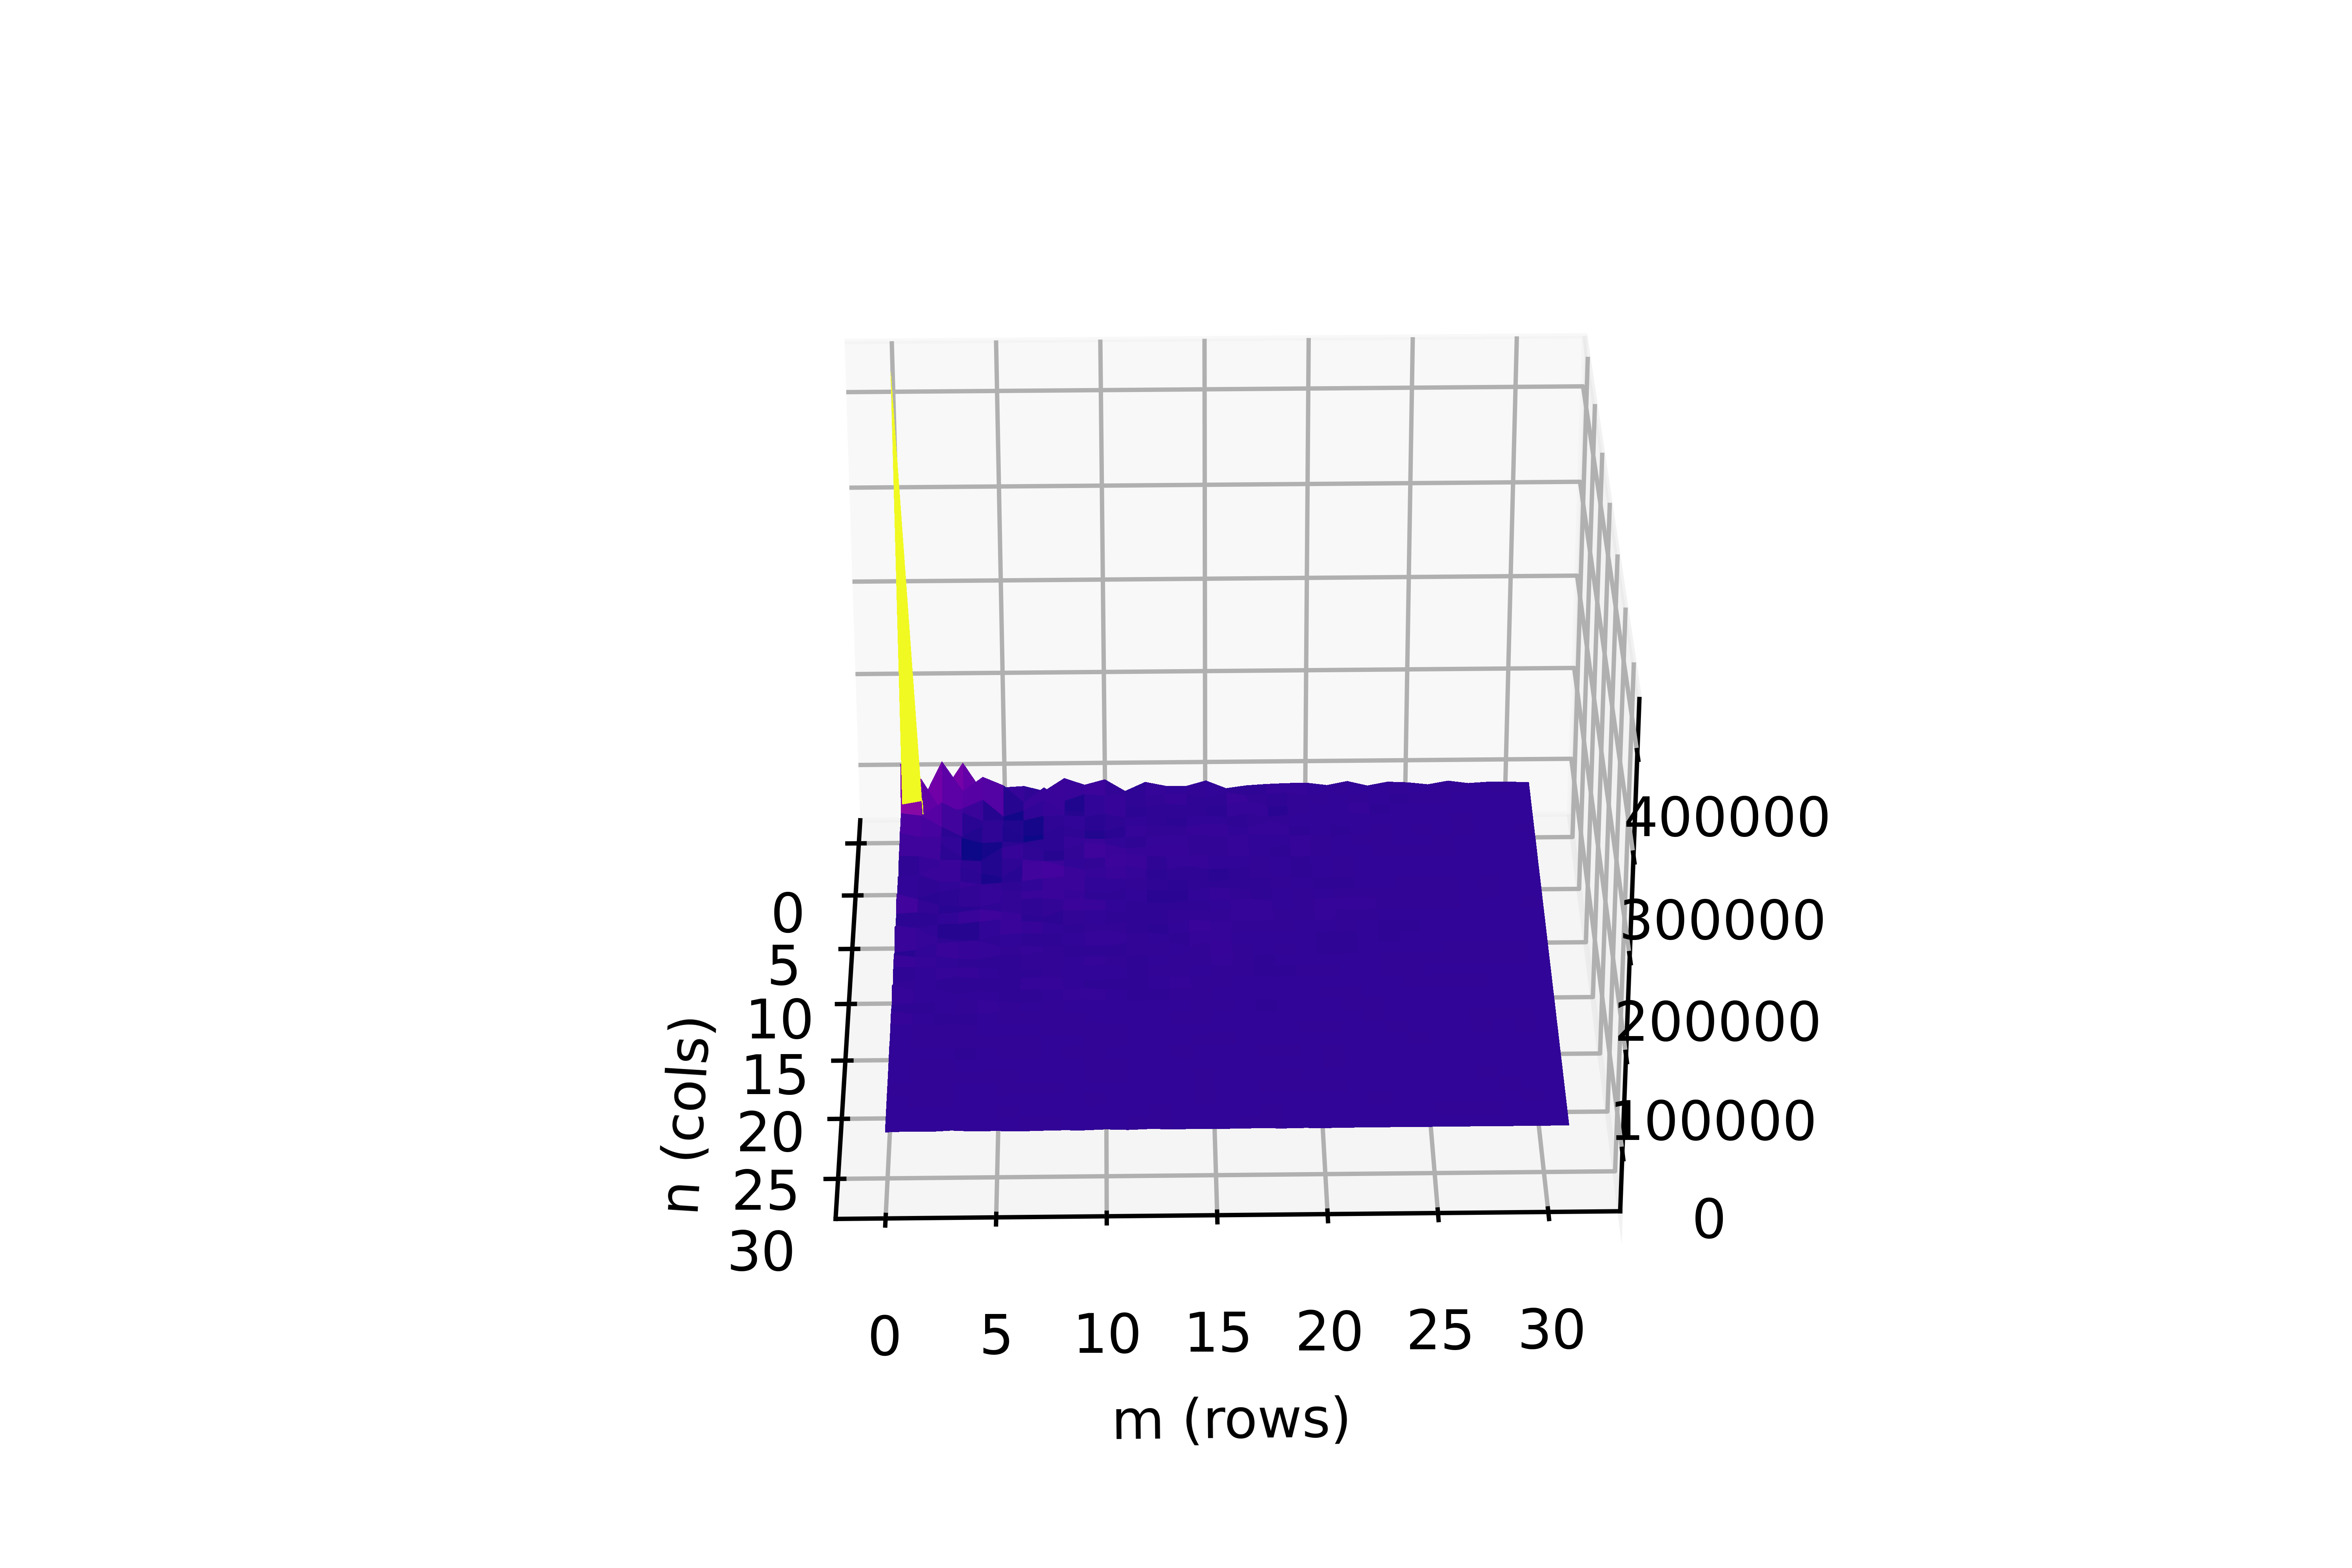
\includegraphics[width=\linewidth]{DCT/dct-2.png}
    \label{img:dct-2}
\end{figure}

DC-коэфициент блока равен среднему всех пикселей в блоке,
взятому с определенным коэффициентом. Удаляя все коэффициенты,
кроме DC, мы можем аппроксимировать блок пикселей их средним
арифметическим. Чем дальше коэффициент располагается от DC,
тем меньше психовизуальной информации он несет для человека,
и тем более незаметные детали изображения он хранит в себе.
Соответственно, основная идея алгоритма состоит в отбрасывании
наименее значимых коэффициентов. Это позволяет производить сжатие
изображения с потерями.

Алгоритм сжатия JPEG работает с каждым каналом отдельно, поэтому для
простоты рассмотрим работу JPEG на изображении в режиме градации серого.
В самом начале своей работы алгоритм разбивает изображение на блоки
8x8 пикселей. К каждому блоку применяется ДКП преобразование,
что равносильно разложению исходной матрицы по базису, состоящему
из 64 функций. Эти 64 функции показаны на рисунке~\ref{img:basis}.
Из этого рисунка видно, что помере отдаления от левого верхнего которая
функции становятся все более рельефными, что объясняет, почему они несут
наиболее мелкие детали изображения. Так же видно, что функция,
соответствующая DC-коэффициенту, представленая плоскостью. Очевидно,
что лучшим константным приближением функции
является ее математическое ожидание.
\begin{figure}[ht]
    \centering
    \caption{Базис ДКП}
    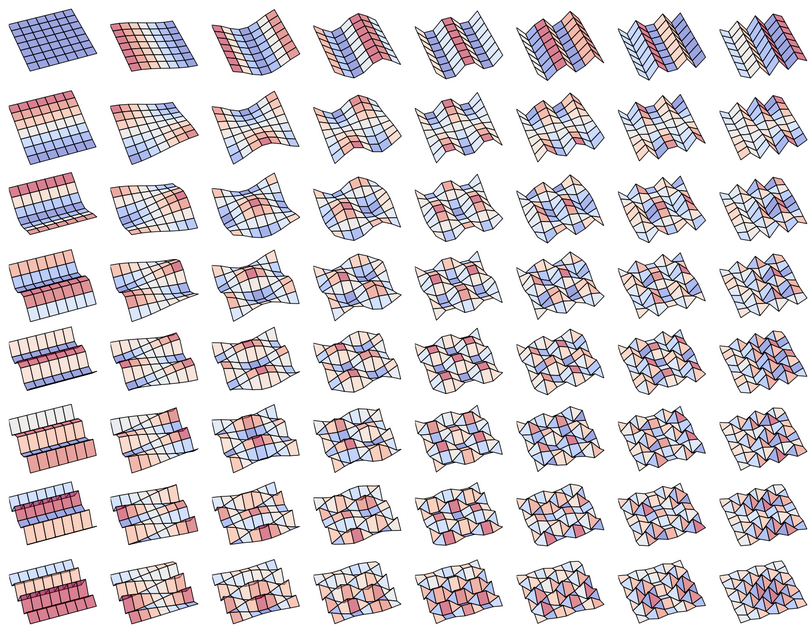
\includegraphics[width=.9\linewidth]{DCT/basis.png}
    \label{img:basis}
\end{figure}
После приминения ДКП преобразования к блоку матрице 8x8
получается другая матрица той же размерности. В соответствии с вышесказанным
эта матрица делится на области низких, средних и высоких частот. В таком порядке
убывает информативность коэффициентов. Это можно увидеть на рисунке~\ref{img:freq}.
\begin{figure}[ht]
    \centering
    \caption{Частотные области ДКП}
    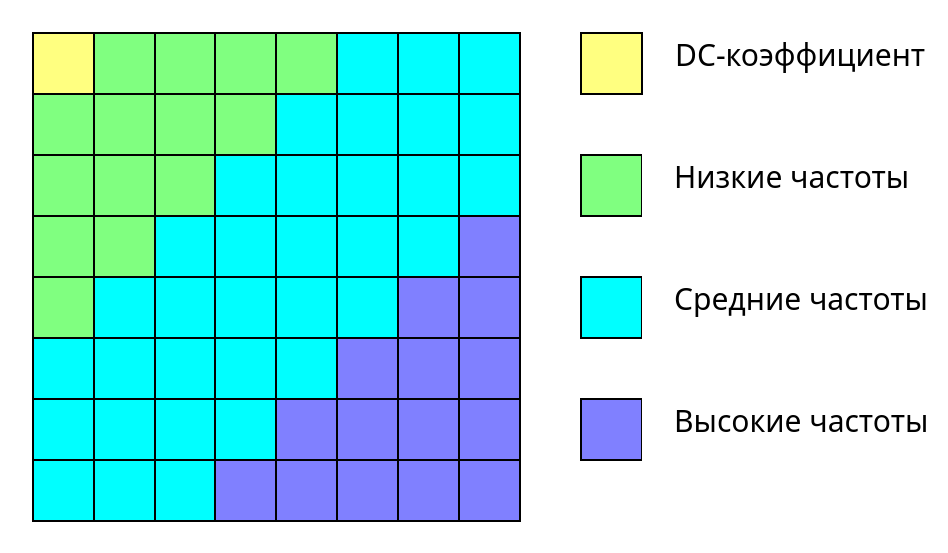
\includegraphics[width=.8\linewidth]{DCT/freq.png}
    \label{img:freq}
\end{figure}
Далее коэффициенты полученной ДКП матрицы квантуются.
Квантование происходит с приминением специальных матриц,
одна из таких матриц представлена в формуле~\ref{eq:q-matrix}.
\begin{equation} \label{eq:q-matrix}
Q=
\begin{bmatrix}
 16 & 11 & 10 & 16 & 24 & 40 & 51 & 61 \\
 12 & 12 & 14 & 19 & 26 & 58 & 60 & 55 \\
 14 & 13 & 16 & 24 & 40 & 57 & 69 & 56 \\
 14 & 17 & 22 & 29 & 51 & 87 & 80 & 62 \\
 18 & 22 & 37 & 56 & 68 & 109 & 103 & 77 \\
 24 & 35 & 55 & 64 & 81 & 104 & 113 & 92 \\
 49 & 64 & 78 & 87 & 103 & 121 & 120 & 101 \\
 72 & 92 & 95 & 98 & 112 & 100 & 103 & 99
\end{bmatrix}.
\end{equation}
Это матрица для 50\% качества, указанная в исходном стандарте JPEG.
Каждый элемент ДКП матрицы делится на коэффициент матрицы квантования,
стоящий в той же позиции. После этого результат округляется. В результате
этой операции обычно бывает так, что многие высокочастотные компоненты
округляются до нуля, а многие из остальных становятся небольшими положительными
или отрицательными числами, для представления которых требуется гораздно меньше бит.

При декодировании происходит обратный процесс --- матрица квантованных коэффициентов
почленное умножается на матрицу квантования, но из-за того, что до этого значения были округлены,
они восстанавливаются с некоторой погрешностью. Чем больше коэффициент квантования,
тем выше будет эта погрешность.

После квантования коэффициенты записываются в специальном зигзагообразном порядке,
показанном на рисунке~\ref{img:zigzag}. Таким образом коэффициенты упорядочиваются
от низких частот к высоким.
\begin{figure}[ht]
    \centering
    \caption{Зигзагообразный порядок}
    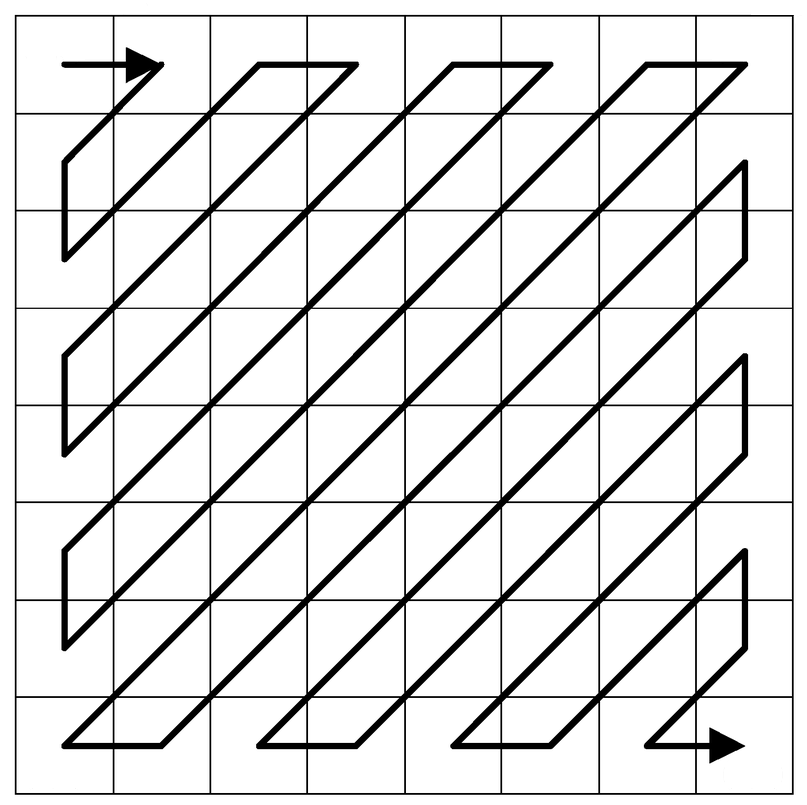
\includegraphics[width=.5\linewidth]{DCT/zigzag.png}
    \label{img:zigzag}
\end{figure}
После этого DC и AC коэффициенты кодируются отдельно.
Поскольку в изображениях часто встречаются
градиентные области, то DC коэффициенты соседних блоков
скорелированны, поэтому первым этапом их кодирования
становится дифференциальная импульсно-кодовая модуляция (ДИКМ).
То есть кодируются не сами коэффициенты, а разница между двумя
соседними коэффициентами.
AC коэффициенты кодируются с помощью кодирования длин серий (КДС).
То есть повторяющиеся символы заменяются на символ и количество его повторов.
После этого к DC и AC коэффициентам применяется энтропийное кодирование с помощью
алгоритма Хаффмана.

Мы разобрали работу алгоритма для одноканального изображения.
В RGB изображениях такой алгоритм применяется к каждому каналу отдельно.
Так же часто кодированию предшествует дополнительный этап,
на котором RGB преобразуется в цветовое пространство
YC\textsubscript{B}C\textsubscript{R}.
Дело в том, что человеческий глаз более чувствителен к перепадам
яркости, чем к перепаду цвета.
В YC\textsubscript{B}C\textsubscript{R} первый канал Y отвечает за яркость,
C\textsubscript{B} и C\textsubscript{R} отвечают за синию и красную компоненты.
После преобразования в YC\textsubscript{B}C\textsubscript{R}
над C\textsubscript{B} и C\textsubscript{R} производится субдискретизация:
каналы разбиваются на небольшие блоки и значения пикселей в этих блоках усредняются.
Таким образом разрешение в этих каналах понижается еще сильнее
и изображение сжимается еще сильнее.
Вся схема алгоритма представлена на рисунке~\ref{img:jpeg-alg}
\begin{figure}[ht]
    \centering
    \caption{Схематичное изображение JPEG}
    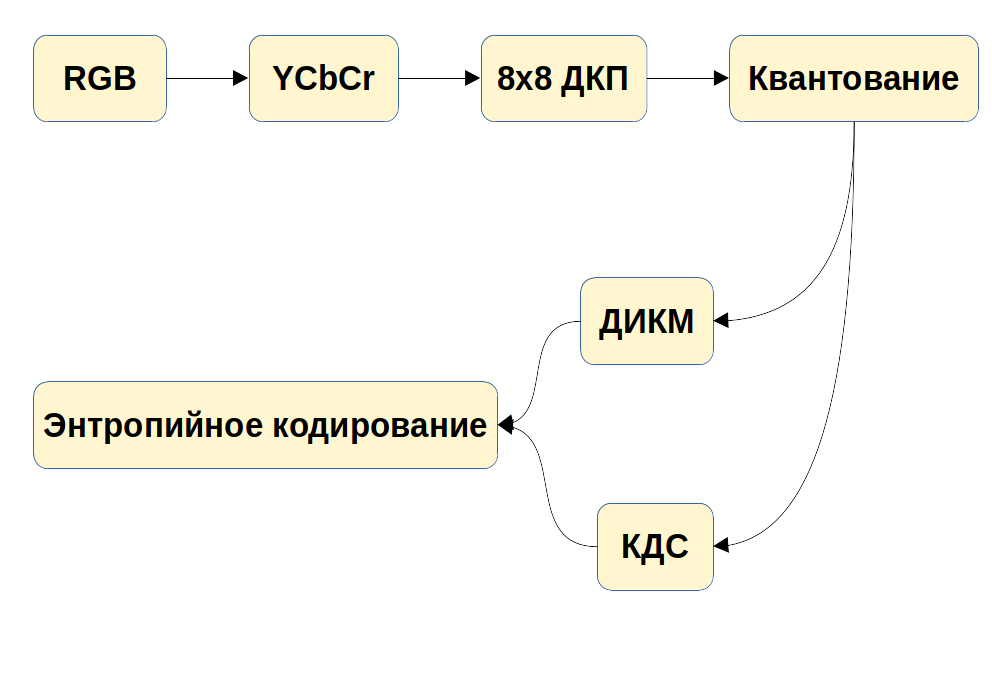
\includegraphics[width=.8\linewidth]{DCT/jpeg-alg.png}
    \label{img:jpeg-alg}
\end{figure}

\section{JSteg}
JSteg --- стеганографический алгоритм, работающий с JPEG файлами.
JSteg во многом опирается на работу кодировщика JPEG. Алгоритмы
кодирования и декодирования JPEG абсолютно симметричны.
JSteg вмешиваетсяв в работу декодировщика, а именно прерывает
его на этапе умножения ДКП коэффициентов на матрицу квантования.
После этого JSteg записывает в упорядоченные зигзагообразным образом
ДКП коэффициенты кодируемую информацию методом LSB. После этого вызывается
кодировщик, который записывает измененные ДКП коэффициенты обратно в JPEG
изображение.

Рассмотрим достоинства и недостатки этого метода.
К доистоинствам можно отнести следующее:
\begin{enumerate}
    \item Низкая вычислительная сложность.
    \item Алгоритм обеспечивает большую вместимость стегосообщений:
    стегосообщение может занимать до 13\% объема контейнера.
    \item Изменения, вносимые в контейнер, незаметны для человеческого глаза.
\end{enumerate}
Но у метода так же есть и существенные недостатки:
\begin{enumerate}
    \item Метод неустойчив к квантованию ДКП коэффициентов.
    Как уже говорилось ранее, операция квантования
    восстанавливает и сохраняет коэффициент с некоторой погрешностью,
    поэтому если открыть в редакторе стегоконтейнер, в котором
    содержится сообщение, закодированное методом JSteg,
    то после пересохранения этого файла сообщение полностью уничтожится. 
    \item Из предыдущих соображения становится ясно, что метод не устойчив
    к сжатию. Это так же обусловлено еще и тем, что при сжатии коэффициенты
    квантования увеличиваются, а значит часть ДКП коэффициентов обнулится,
    а у другой части погрешность восстановления станет еще больше.
\end{enumerate}
Рассмотрим реализацию метода на Python. Код приведен в листинге~\ref{code:jsteg}.
По сути метод представляет собой LSB, только вместо пространственной области
используется спектральная. В данном случае наименее значимый бит меняется
у коэффициентов ДКП изображения, упорядоченных зигзагообразным способом. 
\lstinputlisting[language=Python, label={code:jsteg}, style=simplecode, caption=Реализация JSteg, frame=single]{Code/jsteg.py}

\section{Метод относительной замены величин коэффициентов ДКП}
Этот метод использует идеи, схожие с методами расширения спектра, а именно:
вместо того, чтобы кодировать 1 бит информации в одном коэффициенте ДКП,
метод предлагает кодировать 1 бит информации за счет нескольких коэффициентов ДКП.
Этого можно добиться, кодируя информацию за счет изменения разности между
набором различных коэффициентов ДКП.

Алгоритм Коха-Жао использует 2 коэффициента ДКП.
Формальное описание приводится в алгоритме~\ref{alg:koch-jao}.
Алгоритм декодирования строится симметрично.
Это простейший метод из данного семейства. К доистоинствам
метода можно отнести то, что он устойчив к квантованию ДКП-коэффициентов
и сжатию. Особенно если применять его в паре с помехоустойчив кодироавнием.
Но у метода так же есть и серьезные недостатки:
\begin{enumerate}
    \item Метод вносит заметные искажения в контейнер.
    \item Метод легко детектируется.
\end{enumerate}

\begin{algorithm}[ht!]
    \KwData{Контейнер, Сообщение}
    \KwResult{Заполненный стегоконтейнер}
     $N \leftarrow$ Длина сообщения в битах\;
     $Message \leftarrow$ Бинарное представление сообщения\;
     $DCT$-$blocks \leftarrow$ Массив из блоков ДКП контейнера\;
     $k, l \leftarrow$ Позиция коэффициента ДКП из низкой полосы частот\;
     \For{$i = 1, 2, \ldots, N$}{
         \eIf{$Message[i] = 0$}{
             Сделать $|DCT$-$blocks[i][k][l] - DCT$-$blocks[i][k][l]| < 25$\;
         }{
             Сделать $|DCT$-$blocks[i][k][l] - DCT$-$blocks[i][k][l]| > 25$\;
         }
     }
     $Container \leftarrow$ Новый контейнер, полученный из обратного преобразования ДКП-блоков\;
     \caption{Алгоритм Коха-Жао}
    \label{alg:koch-jao}
\end{algorithm}

Модифицированной версией этого метода является метод Бенгама-Мемона-Эо-Юнга.
Модификации подверглись два направления:
\begin{enumerate}
    \item Встраивание происходит только в наиболее подходящие ДКП-блоки.
    \item Используются не 2, а 3 коэффициента ДКП. Это существенно снижает
    вносимые в контейнер искажения.
\end{enumerate}.
Рассмотрим каждую модификацию в отдельности.

Наиболее подходящие коэффициенты выбираются по следующим признакам:
\begin{enumerate}
    \item Блок не должен иметь слишком резких переходов яркости.
    \item Блок не должен быть слишком монотонным.
\end{enumerate}
Для оценки этих параметров вводится два коэффициента: P\textsubscript{L} и P\textsubscript{H}.
Превышение первого коэффициента или недостижение второго будет указывать на то,
что блок не пригоден для встраивания. Для получения первой оценки нужно проссумировать модуляция
низкочастотных коэффициентов, а для получения второй оценки нужно проссумировать модули высокочастотных
коэффициентов.

Само встраивание происходит в два этапа.
На первом этапе выбираются три коэффициента из низкой полосы частот.
Для обеспечения большой стойкости они могут выбираться псевдослучайно.
На втором этапе коэффициенты модифицируются. Если кодируется 0,
то третий коэффициент должен стать больше первых двух, а если 1,
то третий коэффициент должен стать меньше, соответственно.
Декодирование происходит симметричным образом. Реализацию метода на Python
можно найти в приложении~\ref{appendix-a}.